% !TEX TS-program = xelatex

\documentclass[
	12pt,		%font size
	a4paper,	%paper size
	openright,	%chapters start at odd pages
	oneside,	%uses only one side of the paper
	brazil		%default iphenation idiom
]{abntex2}


\usepackage{tccconfig}
%Concepts
\newcommand{\iot}{IoT}
\newcommand{\iomt}{IoMT}
\newcommand{\middleware}{middleware}
\newcommand{\Middleware}{Middleware}
\newcommand{\smartobj}{\textit{smart object}}
\newcommand{\Smartobj}{\textit{Smart object}}
\newcommand{\smartobjs}{\textit{smart objects}}
\newcommand{\Smartobjs}{\textit{Smart objects}}
\newcommand{\gateway}{gateway}
\newcommand{\Gateway}{Gateway}
\newcommand{\gateways}{gateways}
\newcommand{\Gateways}{Gateways}
\newcommand{\smartphone}{smart\-phone}
\newcommand{\Smartphone}{Smart\-phone}
\newcommand{\smartphones}{smart\-phones}
\newcommand{\Smartphones}{Smart\-phones}
\newcommand{\timestamp}{\textit{timestamp}}
\newcommand{\timestamps}{\textit{timestamps}}
\newcommand{\framework}{framework}

%Technologies
\newcommand{\rfid}{RFID}
\newcommand{\ble}{BLE}
\newcommand{\beacon}{\textit{beacon}}
\newcommand{\Beacon}{\textit{Beacon}}
\newcommand{\beacons}{\textit{beacons}}
\newcommand{\Beacons}{\textit{Beacons}}
\newcommand{\bluetooth}{\textit{bluetooth}}
\newcommand{\Bluetooth}{\textit{Bluetooth}}
\newcommand{\BluetoothLowEnergy}{\textit{Bluetooth Low Energy}}

%Proper noun
\newcommand{\mhub}{M-Hub}
\newcommand{\cddl}{CDDL}
\newcommand{\mhubcddl}{M-Hub/CDDL}
\newcommand{\stwopa}{S2PA}




\titulo{Descoberta e Desconexão de Objetos Inteligentes (\textit{Smart Objects}) em Ambientes Oportunísticos de IoMT}
\autor{Alysson Cirilo Silva}
\data{2019}
\instituicao{Universidade Federal do Maranhão}
\local{São Luis -- MA}
\preambulo{Monografia apresentada ao curso de Ciência da Computação da Universidade Federal do Maranhão, como parte dos requisitos necessários para obtenção do grau de Bacharel em Ciência da Computação.}
\tipotrabalho{Monografia (Graduação)}
\orientador{Francisco José da Silva e Silva}




\begin{document}

\imprimircapa
\imprimirfolhaderosto

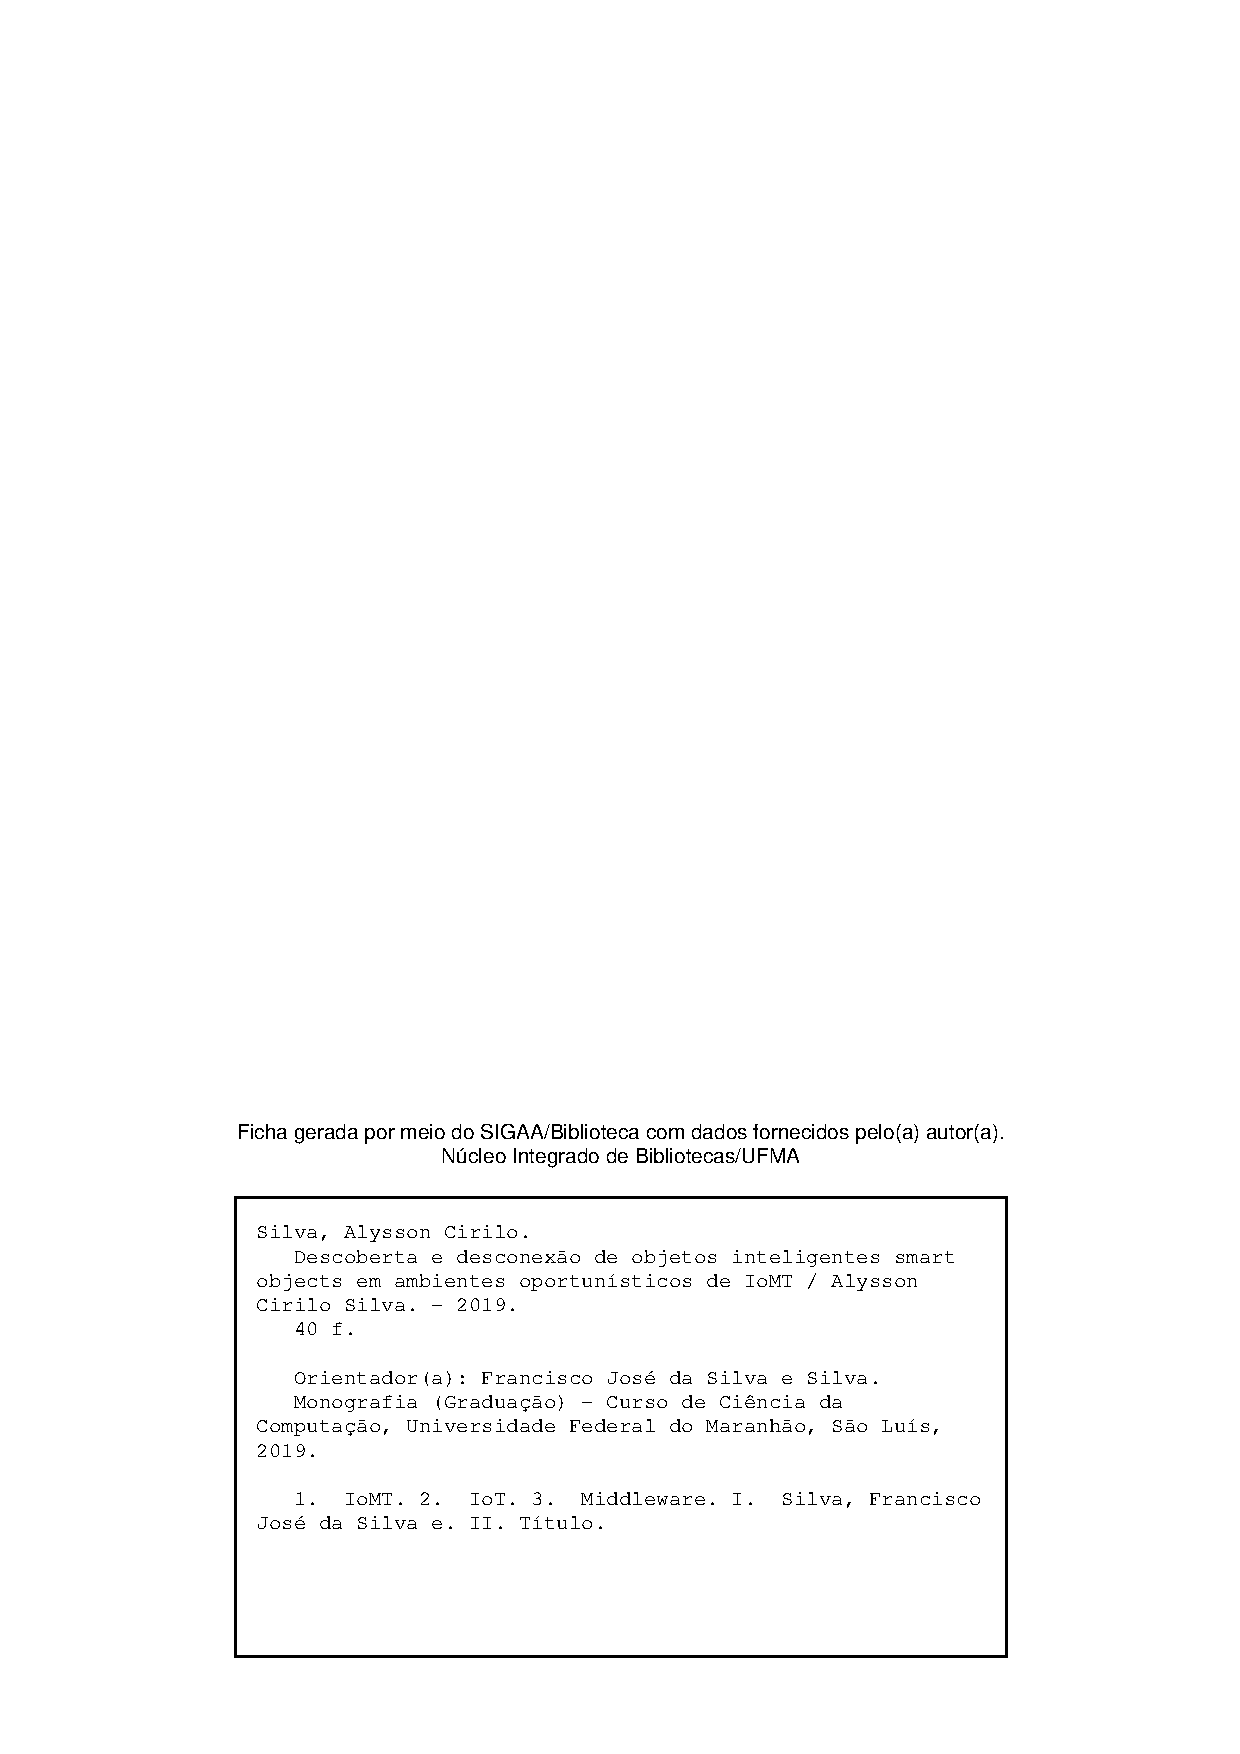
\includepdf{tex/ficha.pdf}
\begin{folhadeaprovacao}

	\begin{center}
		
		{\ABNTEXchapterfont\large\imprimirautor}

		\vspace*{\fill}\vspace*{\fill}
		\begin{center}
		\ABNTEXchapterfont\bfseries\Large\imprimirtitulo
		\end{center}
		\vspace*{\fill}

		\hspace{.45\textwidth}
		\begin{minipage}{.5\textwidth}
		\imprimirpreambulo
		\end{minipage}%
		\vspace*{\fill}

	Trabalho aprovado. \imprimirlocal, \today:
	\end{center}


	\assinatura{\textbf{\imprimirorientador} \\ Orientador} 
	\assinatura{\textbf{Professor} \\ Convidado 1}
	\assinatura{\textbf{Professor} \\ Convidado 2}
	%\assinatura{\textbf{Professor} \\ Convidado 3}
	%\assinatura{\textbf{Professor} \\ Convidado 4}

	\begin{center}

		\vspace*{0.5cm}
		{\large\imprimirlocal}
		\par
		{\large\imprimirdata}
		\vspace*{1cm}

	\end{center}

\end{folhadeaprovacao}

\begin{agradecimentos}
Em primeiro lugar, à Deus, pelo dom da vida.
Ele conhece bem as minhas limitações e me permitiu superá-las em diversos momentos da minha trajetória até aqui.

Agradeço a Universidade Federal do Maranhão (UFMA) e a todos seus professores e colaboradores por me proporcionarem a oportunidade de uma boa educação no curso que faz parte de mim.

Ao meu orientador, Prof. Francisco Silva, pela confiança, disponibilidade, paciência e a tudo que me ensinou.
Também pela oportunidade de participar de projetos tão interessantes e desafiadores.
Será sempre um exemplo que vou seguir.


À minha família pelo apoio, amor e compreensão incondicional que me deram nesta fase tão importante.
Se não fosse por ela não estaria onde estou agora, são a parte mais importante da minha vida e devo tudo a vocês.

À Caroline, minha namorada, por ser um farol que me guia no mar turbulento da vida.
Obrigado por ser uma pessoa tão especial em minha vida, pela compreensão e todos os momentos bons que me deu, não teria conseguido sem seu apoio.
É um imenso prazer para mim dividir um planeta e uma época com você.

Aos membros da banca examinadora, pela dedicação e por aceitarem a missão de avaliar este trabalho.

À todos meus colegas do Laboratório de Sistemas Distribuídos Inteligentes (LSDi) da UFMA, por terem compartilhado comigo tantas horas do dia e ter feito esta experiência muito menos penosa.
Os considero como uma família.

À todos os amigos que encontrei durante essa jornada, nada disso teria valido a pena se não estivessem estado aqui para compartilhar comigo todos os desafios e alegrias.
Obrigado.


\end{agradecimentos}

\begin{epigrafe}
	\vspace*{\fill}
	\begin{flushright}
		\textit{
			The road to wisdom? Well, it's plain\\
			And simple to express:\\
			Err\\
			and err\\
			and err again,\\
			but less\\
			and less\\
			and less.\\
			(Piet Hein)
		}
	\end{flushright}
\end{epigrafe}

\setlength{\absparsep}{18pt} % ajusta o espaçamento dos parágrafos do resumo
\begin{resumo}
	À medida que a \iot se expande no dia a dia e em diversos setores da economia, e dado o caráter opotunístico das interações em ambientes de \iomt, uma extensão da \iot, torna-se claro a importância do mecanismo de detecção de eventos com \smartobjs.
	Em particular, eventos de descoberta, conexão e desconexão com objetos inteligentes se fazem essenciais para uma quantidade considerável de aplicações que interagem com esses dispositivos sem leitura de dados de sensores (\textit{e.g.}, localização \textit{indoor}).
	Este trabalho visa apresentar um módulo de notificação de eventos de descoberta, conexão e desconexão de objetos inteligentes no \middleware \mhubcddl.

	\textbf{Palavras-chave}: \iot. \iomt. \Middleware.
\end{resumo}

\begin{resumo}[Abstract]
	As the \iot expands itself in daily life and in various sectors of economy, and given the opportunistic character of interactions in \iomt environments, an \iot extension, it becomes clear the importance of a smart object event detection mechanism.
	In particular, discovery, connection and disconnection events with smart objects are essential to a considerable number of applications that interact with such devices without the need for sensor data reads (\textit{e.g.}, indoor location).
	This work aims to present a discovery, connection and disconnection event notification module in the \mhubcddl middleware.

	\textbf{Keywords}: \iot. \iomt. \Middleware.
\end{resumo}


\pdfbookmark[0]{\listfigurename}{lof}
\listoffigures*
\cleardoublepage

\pdfbookmark[0]{\listtablename}{lot}
\listoftables*
\cleardoublepage

\tableofcontents
\cleardoublepage

\textual

\chapter{Introdução}

Após a leitura deste capítulo introdutório, o leitor será capaz de entender em qual contexto este trabalho está inserido, assim como compreender o problema e de que forma o trabalho se propõe a combatê-lo.

\section{Contextualização}

\subsection{\iot{}}

A Internet das Coisas (\textit{Internet of Things} -- \iot) é um paradigma de comunicação recente, onde objetos do dia a dia são equipados com equipamentos e protocolos que permitem que se comuniquem com seus usuários e com outros objetos, se tornando parte integral da Internet \cite{Atzori:2010}.  Pode ser definida como a interconexão de sensores e atuadores que fornece a capacidade de compartilhar informações entre plataformas através de um \framework{} unificado \cite{gubbi2013internet}. 

No contexto da \iot{}, as ``coisas'' (do inglês: \textit{things}) são denominados ``\smartobjs'' \cite{bandyopadhyay2011internet}. Seu conceito propõe tornar a Internet ainda mais pervasiva e imersiva, ela promoverá o desenvolvimento de aplicações que utilizarão a grande quantidade e variedade de dados produzidos por esses objetos, de forma a prover serviços para os usuários. 

%colocar isso na Justificativa?
%A medida em que a \iot{} se expande em diversos setores da economia, a demanda para empregar e integrar dispositivos com capacidade de atuação também aumenta. Enquanto que muitos trabalhos lidem com plataformas de \middleware{} que deem suporte ao desenvolvimento de aplicações que necessitem de sensoriamento, pouco foi feito para prover serviços de atuação a nível de \middleware{} \cite{OJIOT_2018v4i1n03_Valim}.

No âmbito desse trabalho, é necessário definir o conceito de \middleware{}, componente essencial para aplicações de \iot{}.
\begin{citacao}
	O \middleware{} é uma camada de software ou conjunto de subcamadas interposta entre os níveis tecnológicos e de aplicação. Sua característica de esconder os detalhes de diferentes tecnologias é fundamental para isentar o programador de problemas que não são diretamente pertinentes para seu foco, que é o desenvolvimento da aplicação específica hablilitada pelas infraestruturas de \iot{} \cite[tradução~nossa]{Atzori:2010}.
\end{citacao}

\subsubsection{\iomt{}}

A \iot{} geralmente lida com \smartobjs{} estáticos, frequentemente presentes na infraestrutura do ambiente, como: sensores de uma sala, leitores \rfid{} de prédios inteligentes, etc. A Internet das Coisas Móveis (Internet of Mobile Things -- \iomt{}) é uma extensão da \iot{} clássica, onde os objetos e os \gateways{} são livres para se locomover, gerando uma maior dinamicidade de interações.

Exemplos de \smartobjs{} móveis incluem: dispositivos vestíveis, veículos, e robôs móveis. Visto o contexto de mobilidade, \smartphones{} são dispositivos adequados para assumir o papel de fornecedor de Internet e serviço de localização---ou seja, um \gateway{}---para \smartobjs{} que tenham disponíveis apenas tecnologias de comunicação sem fio de curto alcance e, dessa forma, não implementam a pilha TCP/IP \cite{talavera2015mobile}.

De acordo com \citeonline{nahrstedt2016internet}, a \iomt{} se diferencia da \iot{} nos seguintes aspectos:
\begin{alineas}

	\item \emph{Contexto}, exemplo:
		
		\begin{alineas}

			\item Onde e com quem o dispositivo móvel se encontra.

		\end{alineas}

	\item \emph{Acesso à Internet e conectividade}, exemplo:
		
		\begin{alineas}

			\item Estado de conexão (conectado/desconectado);
				
			\item Se conectado, em qual rede.

		\end{alineas}

	\item \emph{Disponibilidade de energia}, exemplo:
		
		\begin{alineas}

			\item Onde o dispositivo pode ser recarregado;
				
			\item Quanta energia o aplicativo necessita.

		\end{alineas}

	\item \emph{Segurança e privacidade}, exemplo:
		
		\begin{alineas}

			\item Que tipo de infraestrutura de segurança o dispositivo encontra ao mudar de localização.

		\end{alineas}

\end{alineas}

Dado a dinamicidade característica da \iomt{}, onde a topologia da rede muda constantemente e os \smartobjs{} e \gateways{} interagem de forma oportunística, torna-se claro a necessidade da existência de um mecanismo de notificação que informe aos desenvolvedores de aplicações a ocorrência de eventos de descoberta, conexão e desconexão de \smartobjs{}.

\subsection{\mhubcddl{}}


\section{Caracterização do problema}


\section{Objetivos}


\section{Organização do texto}

O restante deste trabalho é estruturado da seguinte maneira: No \autoref{chap:fundamentacao} será apresentada a fundamentação teórica das tecnologias habilitadoras do trabalho. No \underline{Capítulo 3} a proposta do trabalho é definida. A avaliação da solução proposta é assunto do \underline{Capítulo 4}. As conclusões estão presentes no \underline{Capítulo 4}.


\chapter{Fundamentação teórica} \label{chap:fundamentacao}

Este capítulo visa realizar uma abordagem de toda a fundamentação teórica e tecnológica necessária para o entendimento da solução proposta neste trabalho.

\section{\mhubcddl}

O \mhubcddl é uma composição de um \gateway (\mhub) e um \middleware de \iomt (\cddl). Enquanto o \mhub transforma o dispositivo \android em que está em execução em um \gateway \iot móvel, o \cddl funciona como \middleware provendo serviços locais e remotos de descoberta de provedores de serviços, processamento de eventos complexos, publicação e assinatura de dados e eventos com qualidade de serviço.

As seções seguintes abordarão cada um desses componentes separadamente.

\subsection{\mhub}

O \middleware \mhub pode ser definido, de acordo com \citeonline{talavera2015mobile}, como um serviço de \middleware de \iomt geral executado em um dispositivo móvel pessoal, responsável por descobrir e oportunisticamente conectar à uma miríade de \smartobjs acessíveis apenas através de tecnologias WPAN de curto alcance. Por estar envolvido com cenários de \iomt, este componenete de \software tem que lidar com situações que apresentam muito mais indeterminismo, devido à fatores como a menor garantia de disponibilidade de sensores e atuadores, confiabilidade reduzida, maior volatilidade em conexões, etc.

O \smartphone executando uma intância do \mhub, funciona como \gateway para \smartobjs, fornecendo acesso à internet para dispositivos que não podem se conectar. Outro recurso importante que pode ser explorado pelas aplicações é a habilidade de enriquecer os dados de sensores com dados de contexto obtidos dos sensores internos do \mhub.

\subsubsection{\stwopa}

Para gerenciar a descoberta e conexão com dispositivos que trabalham com diferentes tecnologias de comunicação, além dos sensores internos do \smartphone, o \mhub utiliza o \textit{Short-range Sensing, Presence \& Actuation} (\stwopa), um protocolo que fornece uma \api comum para realizar a comunicação com diferentes tecnologias WPAN.


\chapter{Solução proposta}\label{chap:solucao}

O trabalho em questão tem como objetivo a implementação do mecanismo que propaga os eventos de descoberta, conexão e desconexão que ocorrem no \stwopa do \mhub até a camada de aplicação do \cddl, de forma que os desenvolvedores possam projetar aplicações que se adaptem a tais eventos.
Visto que o \cddl somente exportava à camada de aplicação, eventos de leitura de dados de contexto.

Significando que dentre todos os objetos do tipo \sensordata criados no \stwopa, apenas aqueles com atributo ``\texttt{action}'' assumindo valor ``\texttt{READ}'' geravam eventos no \cddl que podiam ser percebidos pela aplicação (vide \autoref{subsub:s2pa}).

Este fato implica em algumas limitações no desenvolvimento de aplicações.
Imaginando um cenário onde uma aplicação necessite de certos dados providos por um \smartobj--- alocando recursos computacionais para processa-los.
Em uma eventual desconexão com o \smartobj, o fluxo de dados do sensor cessaria de ser entregue à aplicação, contudo, nenhum fluxo ou notificação do evento de desconexão em si seria entregue.
Tal aplicação não poderia decidir se o interrompimento do fluxo de dados se deu: devido a uma mudança na latência do envio de dados por parte do sensor, ou por uma desconexão; não podendo então decidir sobre a necessidade da desalocação de recursos.

Outra classe de aplicações de \iomt que seriam prejudicadas, são aquelas que interagem com \smartobjs no ambiente por outros meios além de conexões.
É o caso de aplicações de localização \textit{indoor} baseadas em \beacons \bluetooth, onde os \beacons são dispostos no interior de ambientes físicos e permanecem realizando \broadcast de sua presença.
Os dispositívos móveis não realizam tentativas de conexão, apenas percebem a presença destes \smartobjs e utilizam a intensidade do sinal capturado no momento.

Vale ressaltar que a implementação também deve permitir que tais eventos possam estar disponíveis para outras aplicações que estejam interessadas, utilizando para isso o \mqtt.
Ou seja---caso configurado desta forma---uma aplicação \mhubcddl pode mudar seu comportamento baseado em eventos que foram disparados a partir de interações entre \smartobjs e \smartphones remotos.

\section{Metodologia} \label{sec:metodologia}

O desenvolvimento do componente de \software foi realizado utilizando a metodologia ágil \textit{Feature-driven development}~\cite{coad:luca:lefebvre:1999}, dividido nas seguintes etapas:

\begin{alineas}
	\item transporte dos eventos gerados no \stwopa para o \cddl;

	\item definição de uma estrutura de tópicos onde os eventos serão publicados pelo \cddl, e posteriormente subscritos pelas aplicações interessadas;

	\item criação de uma \api para o consumo dos eventos.
\end{alineas}

Dentre as características que se considerou importantes, decidiu-se realizar a avaliação de desempenho e acurácia da solução.
As avaliações são realizadas através de simulações de cenários de uso, estes estão descritos no \autoref{chap:avaliacao}.

Como métricas da avaliação de desempenho, mede-se o tempo entre a ocorrência do evento e a sua respectiva notificação na camada de aplicação. Já as métricas de acurácia consistem na verificação da quantidade de notificação de eventos em relação a quantidade de eventos gerados.

\section{Requisitos de \software}

\subsection*{Requisitos funcionais}

Os requisitos funcionais definidos para a solução são:

\begin{alineas}
	\item notificação de eventos de descoberta, conexão e desconexão de \smartobjs para a camada de aplicação do \software;

	\item separação dos fluxos de eventos, provendo uma \api que permita a aplicação registrar interesse em cada tipo de evento individualmente;

	\item permitir que os eventos sejam acessíveis tanto para a aplicação que os gera, quanto para outras aplicações que registrem interesse;

	\item fornecer uma \api assíncrona para o recebimento de cada notificação dos eventos desejados.
\end{alineas}

\section{Implementação}

Esta seção descreve os detalhes de implementação da solução, abordando todos os tópicos descritos na \autoref{sec:metodologia}.

\subsection{Propagação de eventos do \stwopa para o \cddl}

Como descrito na \autoref{subsub:s2pa}, o \mhub encapsula todos os eventos em objetos do tipo \sensordata, estes objetos devem então ser propagados para o \cddl.
O \stwopa comunica-se com o \cddl através do componente \qocevaluator, como pode ser observado na \autoref{fig:mhub-cdll-architecture}~\cite{gomes:2017}.

A comunicação entre os componentes é feita através da biblioteca \eventbus\footnote{\url{http://greenrobot.org/eventbus/}}.
O \eventbus é uma biblioteca de eventos de código livre escrita em Java para a plataforma \android utilizando o padrão \pubsub, fornecendo um mecanismo central de comunicação simplificando a interação entre componentes da aplicação.

O \stwopa foi modificado então para publicar cada \sensordata no \eventbus, enquanto o \qocevaluator registra interesse em receber objetos do tipo \sensordata publicados no \eventbus.
O que efetivamente transfere todos os eventos gerados pelo \stwopa ao \cddl.

\subsection{Separação dos fluxos de eventos}

Como todos os dados publicados pelo \cddl são do tipo \msg, decidiu-se manter este padrão, de forma a manter a retrocompatibilidade e assim continuar suportando as aplicações antigas.
Ao invés de utilizar a estratégia adotada pelo \mhub (utilizar um atributo que identifica que tipo de evento o objeto está representando), adotou-se uma estratégia baseada em orientação a objetos.
Foram criadas três novas classes que herdam os atributos de \msg, são elas:

\begin{alineas}
	\item \objfoundmsg: Para os eventos de descoberta;
	\item \objconnectedmsg: Para os eventos de conexão;
	\item \objdisconnectedmsg: Para os eventos de desconexão.
\end{alineas}

Com esta abordagem é possível utilizar a \api e métodos existentes, valendo-se do mecanísmo de polimorfismo da orientação a objetos.
Ao receber um \sensordata, o \qocevaluator faz o seguinte: identifica, utilizando o atributo \texttt{action}, que tipo de evento ele representa; instancia um objeto de um dos tipos descritos anteriormente; e o publica no \broker \mqtt como um objeto do tipo \msg.

Aplicações que estão interessadas em certo tipo de serviço receberão uma instância de \msg, como ela é superclasse das anteriores, a aplicação pode verificar em tempo de execução se determinado objeto é instância das classes mais especializadas.

\lstinputlisting[float=htb]{code/Polymorphism.java}


\chapter{Avaliação quantitativa}\label{chap:avaliacao}

O objetivo deste capítulo é descrever as avaliações utilizadas na solução proposta. A avaliação tem como objetivo determinar a performance e acurácia do mecanismo de descoberta, conexão e desconexão de \smartobjs{}.

A avaliação será realizada por meio de experimentos, onde a performance será avaliada através da contagem de tempo desde que o \mhub{} efetivamente descobre um objeto até o momento em que a aplicação é informada sobre este evento. A acurácia da solução consistirá na verificação de quantas operações de conexão, desconexão e descoberta geraram eventos correspondentes para a aplicação.

\section{Experimento 1}\label{chap:avaliacao-experimento1}

Este experimento tem como objetivo avaliar a performance e acurácia da solução. Para tal, foi desenvolvido um cenário de uso, onde será possível determinar tais aspectos.

Este cenário de uso consiste em uma casa onde cada cômodo é equipado com um \beacon{} \ble{}, calibrado de forma que o sinal emitido não possa ser detectado fora do cômodo e configurado para emitir 10 anúncios por segundo. Uma pessoa portando um \smartphone{} é instruída a conduzir as atividades do dia a dia nesta residência. Este \smartphone{} executa uma aplicação desenvolvida com o \middleware{} \mhubcddl{} que detecta os anúncios dos \beacons{}, determinando em qual região da casa o indivíduo se encontra.

Ao entrar em um cômodo, o \beacon{} será encontrado pelo \mhubcddl{}, gerando um evento de descoberta no \stwopa{} que deverá ser propagado para a aplicação.

\subsection{Métricas}

Para este experimeto, cada anúncio detectado corresponde a um evento de descoberta gerado pelo \stwopa{}, este evento deve então ser propagado até a aplicação.

A fim de determinar a performance, a aplicação permanece constantemente anotando os \timestamps{} de cada evento de descoberta emitido pelo \stwopa{}, e os \timestamps{} de notificações destes eventos na aplicação---ambos em milisegundos. O primeiro \timestamp{} é subtraído do segundo de forma a calcular o tempo de propagação dos eventos de descoberta, que será de agora em diante referido como $TP_{descoberta}$ e calculado da seguinte forma. 

\begin{equation}
	\label{equ:performance-discovery}
	TP_{descoberta} = TS_{descoberta,app} - TS_{descoberta,\stwopa{}}
\end{equation}

Onde $TS_{descoberta,app}$ e $TS_{descoberta,\stwopa{}}$ se referem ao \timestamp{} de uma notificação de descoberta na aplicação e ao \timestamp{} do evento de descoberta gerado pelo \stwopa{}, respectivamente.

Para avaliar a acurácia é realizada uma comparação entre a quantidade de eventos que foram gerados e quantas notificações foram entregues à aplicação, e será calculada da seguinte maneira.

\begin{equation}
	\label{equ:acuracy}
	Acur\acute{a}cia = \frac{EventosGerados - |EventosGerados - EventosNotificados|}{EventosGerados}
\end{equation}

Onde $EventosGerados$ e $EventosNotificados$ se referem à quantidade de eventos gerados no \stwopa{} e à quantidade de notificações desses eventos que chegaram à aplicação, respectivamente.

A \autoref{tab:generated-events-1} mostra os valores do termo $EventosGerados$ na \autoref{equ:acuracy}, estes valores serão posteriormente comparados com a quantidade de eventos notificados para calcular a acurácia.

\begin{table}[htb]
	\begin{center}
		\IBGEtab{
			\caption{Quantidade de eventos que serão gerados no experimento 1}
			\label{tab:generated-events-1}
		}{
			\begin{tabular}{lc}
				\toprule
				& \textbf{$EventosGerados$}	    \\
				\midrule \midrule
				\textbf{Eventos de descoberta}	& 34814	    \\
				\textbf{Eventos de conexão}	& 0	    \\
				\textbf{Eventos de desconexão}	& 0	    \\
				\bottomrule
			\end{tabular}
		}{
			\fonte{\autoriapropria}
		}
	\end{center}
\end{table}

\subsection{Simulação dos \beacons{}}\label{chap:avaliacao-simulacao-beacons}

O experimento descrito na \autoref{chap:avaliacao-experimento1} foi simulado utilizando um \dataset{}, esta seção descreve como este \dataset{} foi utilizado para simular a detecção dos \beacons{}. Os dados utilizados para a simulação do experimento 1 foram obtidos do \dataset{} disponibilizado por \citeonline{byrne2018residential}\footnote{O \dataset{} pode ser obtido em \cite{byrne2019dataset}}. Neste trabalho os autores instruíram que participantes conduzissem suas rotinas diárias em casa, enquanto sua localização na residência era monitorada.

O chão dos cômodos das casas foi marcado com etiquetas, cada etiqueta é uma imagem binária que codifica um número inteiro, e este, único para cada uma das etiquetas. Os participantes são equipados com uma câmera na região do torso que aponta em direção ao chão, detectando e interpretando qual etiqueta está visível no momento, e deste modo, identificando em qual cômodo o participante se encontra.

No trabalho citado, o autor realizou o experimento em 4 residências distintas, e estas, foram denotadas de ``\texttt{Residence A}'', ``\texttt{Residence B}'', ``\texttt{Residence C}'' e ``\texttt{Residence D}''. Para cada residência, o experimento foi conduzido múltiplas vezes, e cada um denominado de ``\texttt{living\_1}'', ``\texttt{living\_2}'', ``\texttt{living\_3}'', \dots{}, ``\texttt{living\_n}''.


A fim de maximizar a quantidade de eventos de descoberta, foi utilizado os dados do experimento ``\texttt{living\_2}'' da casa ``\texttt{Residence D}'' pois este experimento possui um dos maiores tempos de monitoramento e quantidade de entrada em cômodos. Os dados deste experimento consistem de 58 minutos de monitoramento de um indivíduo em uma casa de 10 cômodos. Os dados possuem uma resolução média de aproximadamente 11 medições por segundo.

Informações referentes à distribuição da quantidade de vezes em que o indivíduo visita um quarto estão sumarizadas na \autoref{fig:dataset-histogram}.

\begin{figure}[htb]
	
	\begin{center}
		
		\caption{\label{fig:dataset-histogram}Frequência de entrada por cômodo}
		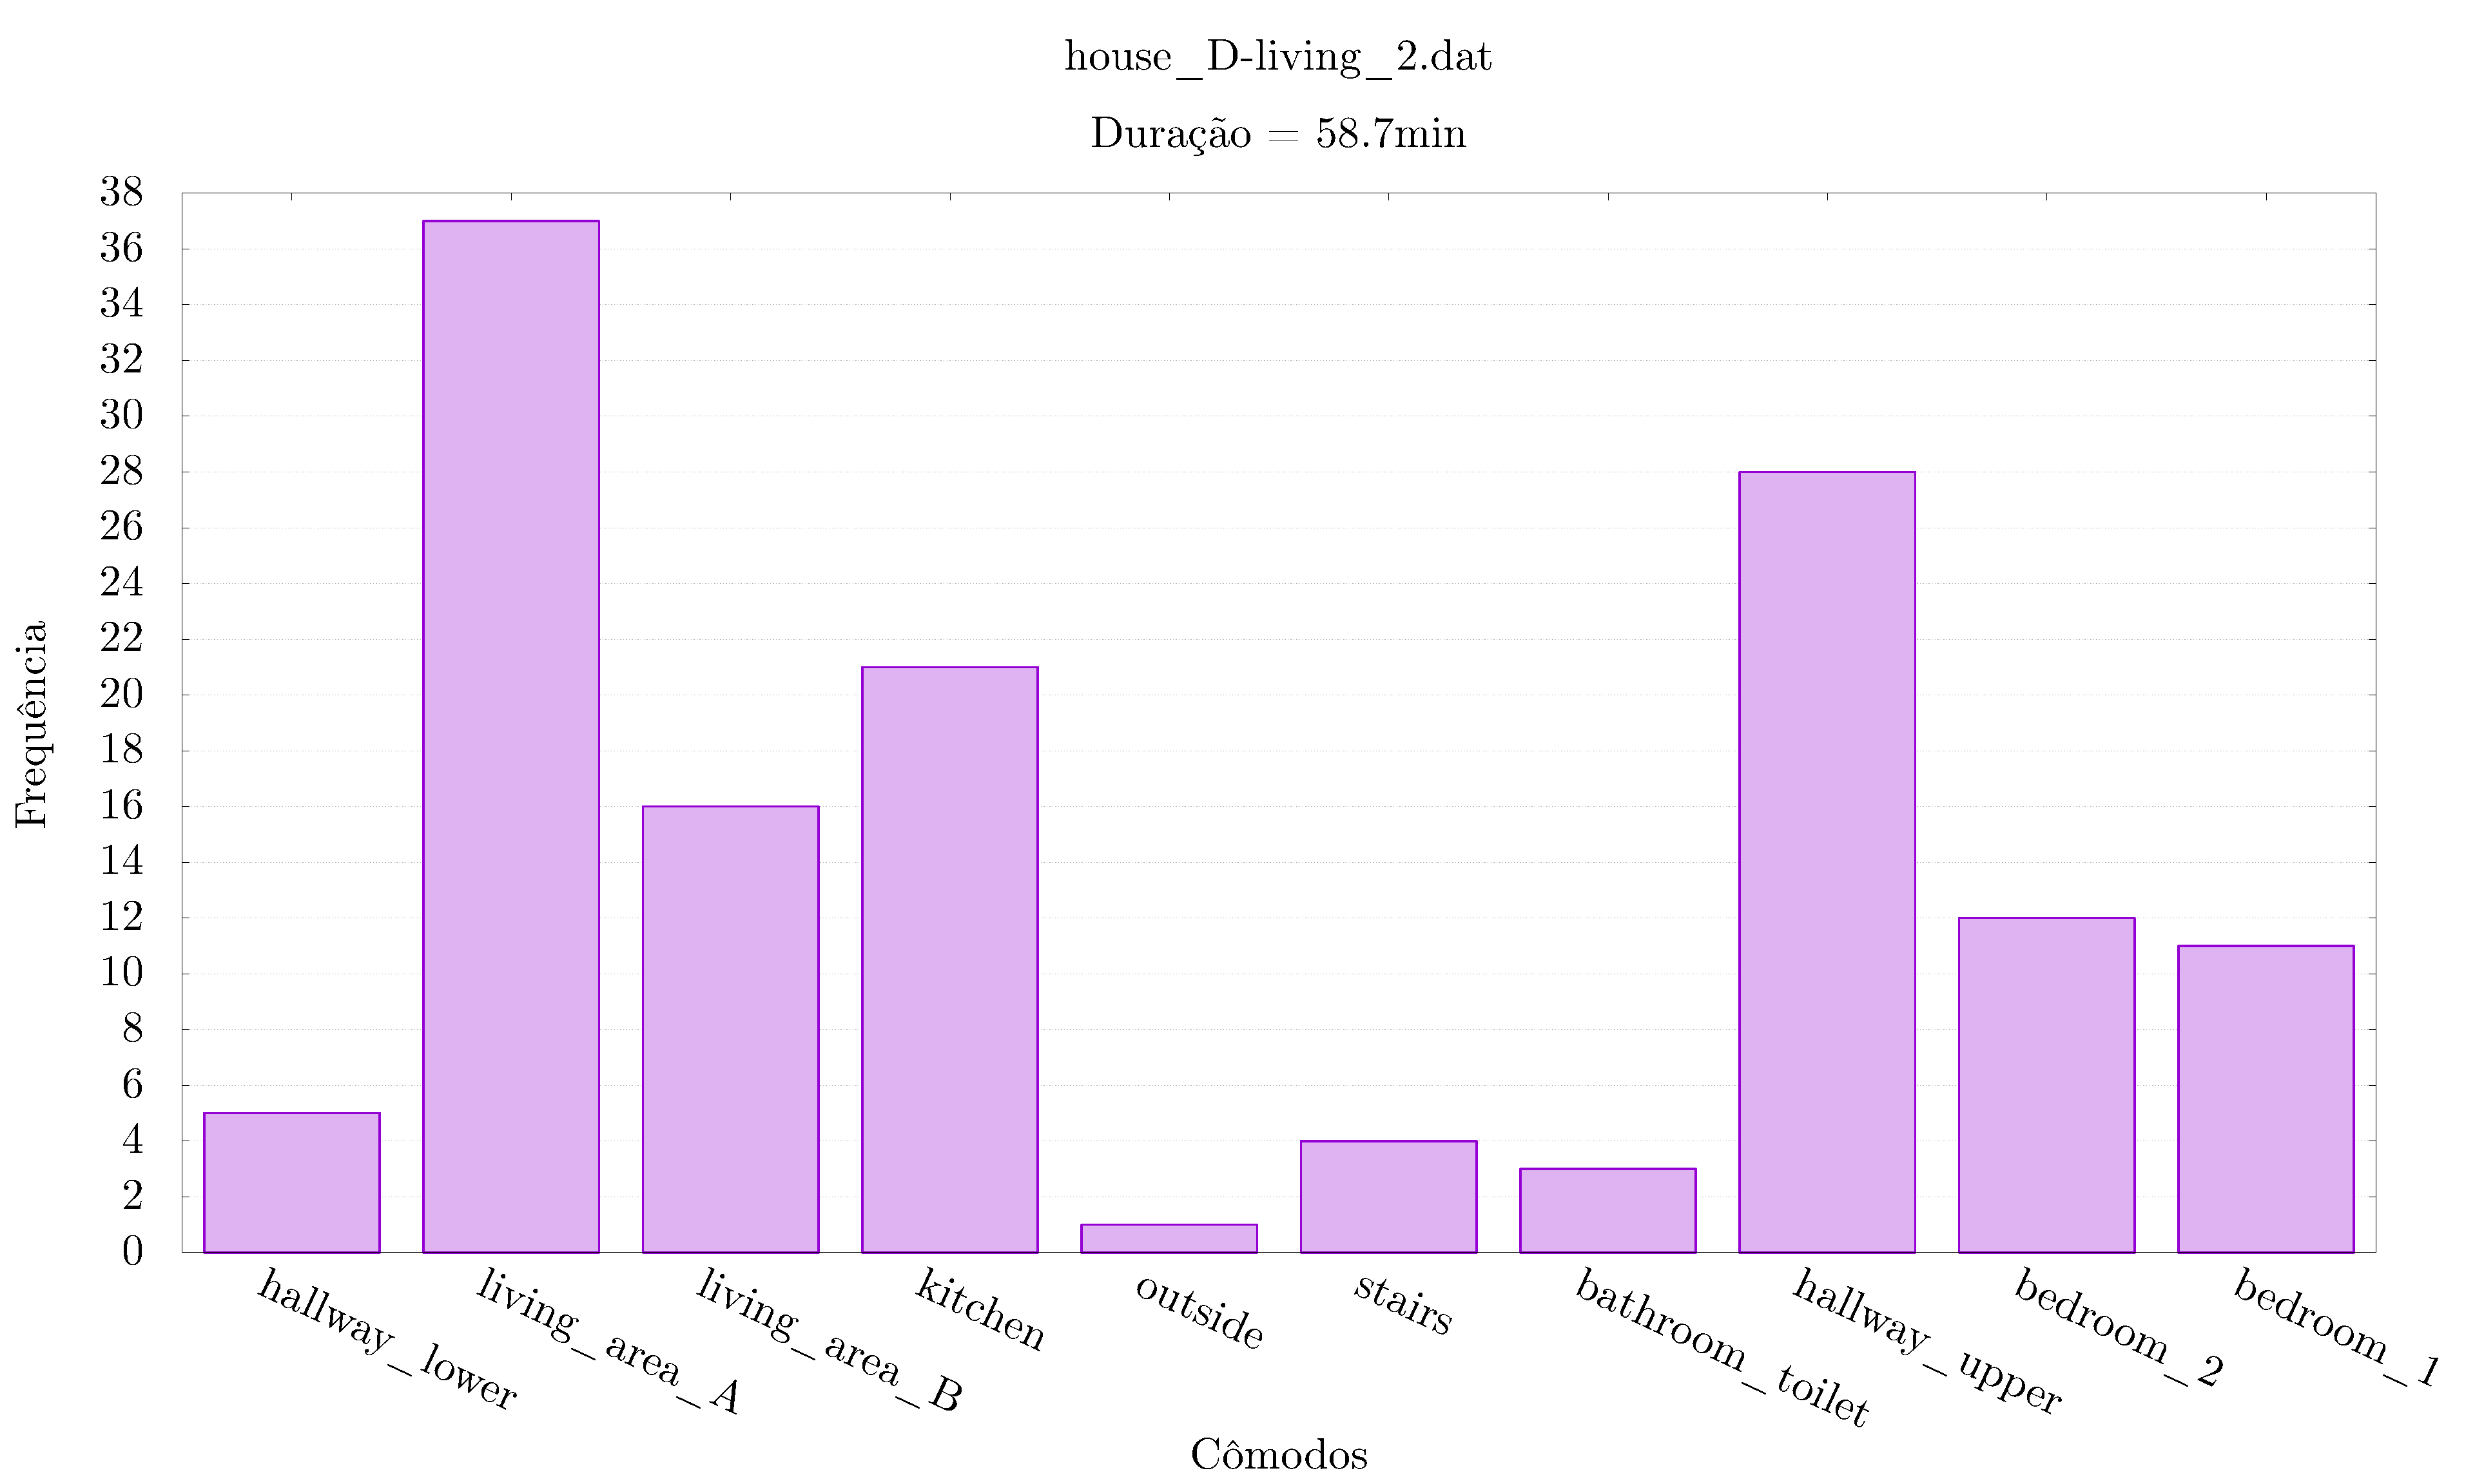
\includegraphics[scale=0.246]{img/dataset-histogram}
		\fonte{\autoriapropria{}}
		
	\end{center}

\end{figure}

O \dataset{} original é composto principalmente por um arquivo de texto que contém em cada linha uma representação de um momento no decorrer do experimento. Entre os dados contidos por linha, destaca-se o \timestamp{} da medição e a etiqueta detectada naquele instante. 

Realizou-se um pré-processamento no \dataset{} de forma a facilitar a utilização dos dados para fim da simulação, gerando um arquivo contendo 3 valores separadas por espaço em que cada linha representa o instante em que o participante entrou e permaneceu contínuamente em um cômodo. Os 3 valores são: um identificador numérico do cômodo, o nome do cômodo e o \timestamp{} em que o indivíduo entrou naquele cômodo, como pode ser visto no \autoref{lst:preprocessed-dataset}.

\begin{center}
	
	\begin{lstlisting}[caption={Parte do \dataset{} pré-processado}, label=lst:preprocessed-dataset]
		#room	room-name	timestamp(seconds)
		2	living_area_A	485.352
		1	hallway_lower	506.273
		6	stairs		513.380
		8	hallway_upper	519.319
		10	bedroom_1	526.159
		8	hallway_upper	561.328
		7	bathroom_toilet	565.832
		8	hallway_upper	628.495
		9	bedroom_2	632.065
	\end{lstlisting}
	
\end{center}

Como descrito anteriormente, cada um dos 10 cômodos possui um \beacon{} \ble{}, configurados para emitir 10 anúncios por segundo. É esperado, então,  que o aplicativo detecte um anúncio a cada 0.1 segundo em que o participante permanece em um cômodo. 

Utilizando o \dataset{} já descrito, a cada momento em que o participante entra em determinado cômodo, calcula-se quantos anúncios o \beacon{} daquele cômodo transmitirá durante o tempo de permanência no local, o cálculo é apresentado a seguir.

\begin{equation}
	anuncios = \frac{tempoPermanencia}{0.1} 
\end{equation}

Onde $tempoPermanencia$ denota o tempo que o indivíduo permaneceu no cômodo. Os anúncios são então repoduzidos a cada intervalo de 0.1 segundo. Com isso foi possível calcular previamente os valores da \autoref{tab:generated-events-1}.

\subsection{Coleta das métricas de performance}

Na \autoref{img:performance-annotation} é possível observar onde os \timestamps{} utilizados na avaliação de performance são anotados. Ambos os \timestamps{} são denotados na imagem por um cronômetro. Na imagem, $T0$ e $T1$ são equivalentes à $TS_{descoberta,\stwopa{}}$ e $TS_{descoberta,app}$ da \autoref{equ:performance-discovery}.

\begin{figure}[htb]
	
	\begin{center}

		\caption{\label{img:performance-annotation}Componentes onde há a captura de \timestamps{}}
		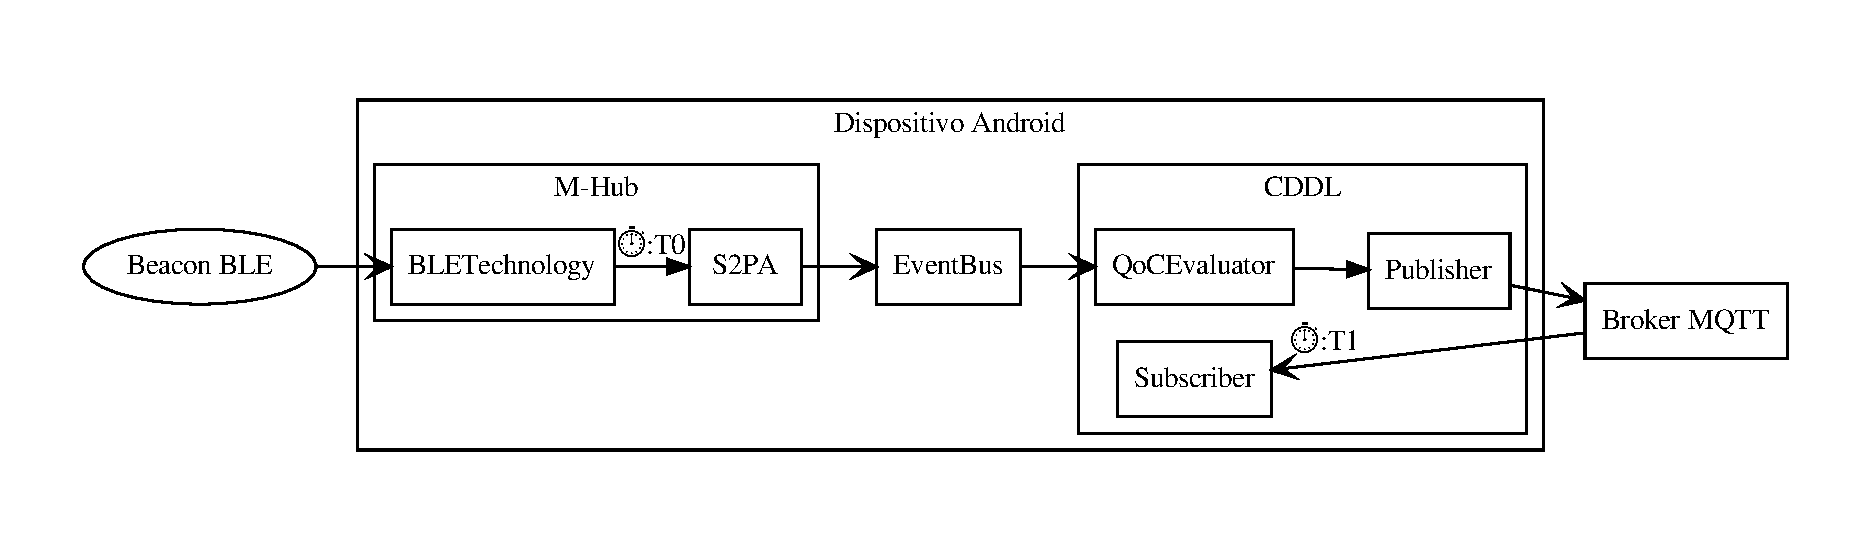
\includegraphics[scale = 0.50]{img/performance-annotation}
		\fonte{\autoriapropria{}}

	\end{center}
	
\end{figure}

\subsection{Recursos computacionais}

O experimento descrito foi executado em um \smartphone{} Lenovo Moto Z Play, com processador de 8 núcleos e 2GHz, e 3GB de memória RAM.

Também foi utilizado uma máquina virtual como \broker{} \mqtt{}, esta máquina executa o sistema operacional Ubuntu 16.04.4 LTS, possui processador de 2 núcleos com 2.5GHz e 4GB de memória RAM.

\section{Experimento 2}

O segundo experimento visa avaliar o desempenho e acurácia da solução proposta, entretanto levando em consideração também os eventos de conexão e desconexão que não foram analisados no primeiro experimento. O experimento consiste em um cenário de uso composto por uma casa equipada com um sistema multimídia na sala de estar que possibilita que \smartphones{} se conectem a ele através de \bluetooth{}, onde o conteúdo da televisão se adapta de acordo com os usuários que estão presentes na sala, e a interação com as aplicações da televisão digital acontece através do \smartphone{}.

O sistema multimídia pode ter ciência de qual usuário está presente através dos \smartphones{} conectados no momento, pois ele armazena a relação dos moradores da residência com seus respectivos \smartphones{}.

Uma aplicação android foi desenvolvida com o \middleware{} \mhubcddl{} que permanece ativamente procurando e se conectando ao sistema multimídia no ambiente. Ao entrar na sala de estar o sistema multimídia é encontrado e em seguida a conexão é estabelecida. Quando o usuário sai da sala de estar a conexão é desfeita. 

\subsection{Métricas}

Para o experimento 2, a todo momento em que o participante entra na sala de estar acontece interações entre o aplicativo e o sistema multimídia, essas interações são compostas de um evento de descoberta, seguido por um evento de conexão. Ao sair do quarto um evento de desconexão é também gerado. Cada um desses eventos são gerados pelo \stwopa{} e notificados posteriormente à aplicação.

As avaliaçãos de desempenho e acurácia deste cenário de uso são análogas às descritas para o experimento 1, com a exceção de que eventos de conexão e desconexão também fazem partes das medições.

A \autoref{equ:performance-discovery} será utilizada para avaliar a performance da notificação de eventos de descoberta. A performance da notificação dos eventos de conexão e desconexão serão os tempos de propagação de tais eventos até a aplicação, e denotados como $TP_{conexao}$ e $TP_{desconexao}$ respectivamente.

\begin{equation}
	\label{equ:performance-connection}
	TP_{conexao} = TS_{conexao,app} - TS_{conexao,\stwopa{}}
\end{equation}

\begin{equation}
	\label{equ:performance-disconnection}
	TP_{desconexao} = TS_{desconexao,app} - TS_{desconexao,\stwopa{}}
\end{equation}

Onde $TS_{conexao,\stwopa{}}$ e $TS_{desconexao,\stwopa{}}$ são os \timestamps{} de quando os eventos de conexão e desconexão são gerados no \stwopa{}. Já $TS_{conexao,app}$ e $TS_{desconexao,app}$ são os \timestamps{} de quando esses eventos são entregues à aplicação.

Para medir a acurácia será utilizado a \autoref{equ:acuracy}. A \autoref{tab:generated-events-2} sumariza os resultados esperados para o experimento.

\begin{table}[htb]
	\begin{center}
		\IBGEtab{
			\caption{Quantidade de eventos que serão gerados no experimento 2}
			\label{tab:generated-events-2}
		}{
			\begin{tabular}{lc}
				\toprule
				& \textbf{$EventosGerados$}		\\
				\midrule \midrule
				\textbf{Eventos de descoberta}	& 37	\\
				\textbf{Eventos de conexão}	& 37	\\
				\textbf{Eventos de desconexão}	& 37	\\
				\bottomrule
			\end{tabular}
		}{
			\fonte{\autoriapropria}
		}
	\end{center}
\end{table}

\subsection{Simulação do sistema multimídia}

Para este experimento foi feita uma simulação de um indivíduo andando em uma residência, foram utilizados os dados do \dataset{} descrito na \autoref{chap:avaliacao-simulacao-beacons} para esta simulação.

Escolheu-se também o experimento ``\texttt{living\_2}'' da casa ``\texttt{Residence D}'' por fornecer um dos maiores tempos de monitoramento do participante juntamente com a maior quantidade de visitas à sala de estar. Será utilizado apenas a parte do \dataset{} referentes à entradas no cômodo denotado como ``\texttt{living\_area\_A}'' na \autoref{fig:dataset-histogram}, pois este cômodo foi escolhido como a sala de estar onde o sistema multimídia se localiza.

\section{Resultados}

\begin{table}[htb]
	\begin{center}
		\IBGEtab{
			\caption{Quantidade de eventos notificados no experimento 1}
			\label{tab:generated-events-1-results}
		}{
			\begin{tabular}{lccc}
				\toprule
				& \textbf{$EventosGerados$} & $EventosNotificados$ & $Acur\acute{a}cia$(\%)	\\
				\midrule \midrule
				\textbf{Eventos de descoberta}	& 34814	& 34811	& 99.99				\\
				\textbf{Eventos de conexão}	& 0	& 0	& ---				\\
				\textbf{Eventos de desconexão}	& 0	& 0	& ---				\\
				\bottomrule
			\end{tabular}
		}{
			\fonte{\autoriapropria}
		}
	\end{center}
\end{table}


\begin{table}[htb]
	\begin{center}
		\IBGEtab{
			\caption{Quantidade de eventos notificados no experimento 2}
			\label{tab:generated-events-2-results}
		}{
			\begin{tabular}{lccc}
				\toprule
				& \textbf{$EventosGerados$} & $EventosNotificados$ & $Acur\acute{a}cia$(\%)	\\
				\midrule \midrule
				\textbf{Eventos de descoberta}	& 37	& 37	& 100				\\
				\textbf{Eventos de conexão}	& 37	& 37	& 100				\\
				\textbf{Eventos de desconexão}	& 37	& 37	& 100				\\
				\bottomrule
			\end{tabular}
		}{
			\fonte{\autoriapropria}
		}
	\end{center}
\end{table}


\chapter{Conclusões} \label{chap:conclusao}


\postextual

\bibliography{bib/biblio}

\end{document}
